\documentclass[conference]{IEEEtran}
\IEEEoverridecommandlockouts
% The preceding line is only needed to identify funding in the first footnote. If that is unneeded, please comment it out.
\usepackage{cite}
\usepackage{amsmath,amssymb,amsfonts}
\usepackage{algorithmic}
\usepackage{graphicx}
\usepackage{textcomp}
\usepackage{xcolor}
\usepackage{booktabs}
\def\BibTeX{{\rm B\kern-.05em{\sc i\kern-.025em b}\kern-.08em
    T\kern-.1667em\lower.7ex\hbox{E}\kern-.125emX}}
\begin{document}



\title{Códigos de linha}

\author{
\IEEEauthorblockN{Luís Gustavo Werle Tozevich, Jaime Antonio Daniel Filho, Guilherme M. Einloft e Guilherme Brizzi}
\IEEEauthorblockA{
Curso de Ciência da Computação \\
Universidade Federal de Santa Maria (UFSM) \\
Santa Maria, Brasil \\
lgtozevich@inf.ufsm.br, jafilho@inf.ufsm.br, guieinloft@proton.me, gbrizzi@inf.ufsm.br
}
}

\maketitle


\begin{abstract}
Este trabalho aborda os códigos de linha 4B3T, 8B6T e 4D-PAM5, explorando suas características técnicas, contextos de aplicação e funcionamento. Detalha-se o mapeamento, vantagens (como eficiência espectral) e limitações (complexidade, sensibilidade a ruído) de cada código, destacando seu papel em sistemas de comunicação modernos e legados. Conclui-se que a escolha de um código de linha depende de fatores como infraestrutura existente, requisitos de largura de banda e restrições tecnológicas.
\end{abstract}

\begin{IEEEkeywords}
Códigos de linha, comunicação de dados, transmissão digital.
\end{IEEEkeywords}

\section{Introdução}

A transmissão de dados digitais em sistemas de comunicação constitui um dos pilares fundamentais para o desenvolvimento tecnológico contemporâneo. Nesse contexto, os códigos de linha emergem como elementos essenciais para viabilizar a comunicação eficiente entre dispositivos digitais, representando um campo de estudo relevante na interseção entre Ciência da Computação e Engenharia de Telecomunicações.

Os códigos de linha, também denominados códigos de transmissão, são métodos de representação de sinais binários através de formas de onda elétricas ou ópticas, permitindo a transmissão de informação digital através de meios físicos. Esses códigos definem como os bits são convertidos em sinais elétricos ou ópticos para transmissão, estabelecendo um mapeamento entre sequências binárias e níveis de tensão, corrente ou potência óptica (SKLAR, 2001).

A implementação adequada de códigos de linha atende a objetivos críticos em sistemas de comunicação digital. Entre estes, destacam-se: (i) sincronização eficiente entre transmissor e receptor, permitindo a recuperação correta do relógio de bits; (ii) detecção e, em alguns casos, correção de erros de transmissão; (iii) otimização do espectro de frequência do sinal transmitido; (iv) minimização da interferência intersimbólica; e (v) redução da componente DC do sinal, facilitando a implementação dos circuitos de acoplamento.

A escolha de um código de linha específico para determinada aplicação implica em um compromisso entre diversos fatores, como eficiência espectral, complexidade de implementação, robustez contra ruído, e requisitos de largura de banda. Esta decisão influencia diretamente o desempenho global do sistema de comunicação, impactando em aspectos como taxa de erro de bits (BER), consumo de energia e viabilidade econômica.

O presente trabalho tem como objetivo analisar e comparar três padrões específicos de códigos de linha que não foram abordados no conteúdo programático regular da disciplina de Comunicação de Dados na Universidade Federal de Santa Maria. Os códigos 4B3T, 8B6T e 4D-PAM5 serão definidos e detalhados nas seções subsequentes, onde serão analisadas suas propriedades, vantagens, desvantagens e aplicações práticas.



\section{Código de linha 4B3T}

\subsection{Contextualização e aplicações}

O código de linha 4B3T (four binary, three ternary), também conhecido como MMS (Modified Monitoring State) 43, foi desenvolvido como solução eficiente para a transmissão de dados em sistemas de acesso básico da Rede Digital de Serviços Integrados (ISDN), especialmente no contexto de transmissão sobre cabos de cobre existentes. Este esquema de codificação surgiu para permitir taxas de transmissão de 160 kbps (2B+D) sobre par trançado sem necessidade de amplificação, atendendo aos requisitos de simplicidade, eficiência espectral e imunidade a ruído.

A adoção do 4B3T é notavelmente encontrada nas interfaces U da ISDN, padronizadas pelas recomendações ITU-T, como a I.430, onde se especifica a codificação de quatro bits binários em três símbolos ternários (-1, 0, +1) para otimizar a utilização do espectro. Países europeus, como Alemanha e França, implementaram extensivamente este padrão em suas redes públicas, garantindo interoperabilidade e eficiência em infraestruturas já implantadas.

Além da ISDN, o conceito de codificação multibits-para-multiníveis, exemplificado pelo 4B3T, inspirou o desenvolvimento de esquemas de transmissão posteriores, como os utilizados em tecnologias xDSL (Digital Subscriber Line), evidenciando sua relevância histórica e técnica na evolução das comunicações sobre par metálico.

\subsection{Funcionamento}

O código 4B3T realiza o mapeamento de blocos de quatro bits em três símbolos ternários, cada um podendo assumir valores -1, 0 ou +1 (ETSI, 1996). Esta abordagem reduz a taxa de símbolos transmitidos em comparação com codificações binárias simples, otimizando a largura de banda necessária e melhorando a imunidade a distorções de alta frequência.

A eficiência do 4B3T advém de seu mapeamento balanceado, que procura minimizar o deslocamento DC (componente contínua) e a interferência intersimbólica (ISI). Para isso, são aplicados algoritmos de codificação que asseguram que a sequência de símbolos tenha uma média próxima de zero ao longo do tempo, uma propriedade crítica para a transmissão confiável em cabos sem amplificação e com acoplamento por transformadores.

No processo de codificação, cada grupo de 4 bits de entrada é convertido em uma sequência de 3 ternários, segundo uma tabela de mapeamento pré-definida (Tabela \ref{tab:4b3t}). Nesta tabela, seis dos grupos de 4 bits (\texttt{0001}, \texttt{0111}, \texttt{0100}, \texttt{0010}, \texttt{1011}, \texttt{1110}) possuem uma sequência neutra (com DC offset 0), enquanto as restantes possuem uma com DC offset positivo e outra com DC offset negativo. A próxima sequência na tabela é escolhida com base no DC offset acumulado, buscando sempre mantê-lo próximo de 0. Na recepção, a sequência de três símbolos é decodificada para recuperar os quatro bits originais, utilizando circuitos digitais de baixa complexidade.

\begin{table}[ht]
\centering
\caption{Tabela de codificação 4B3T (ISDN)}
\renewcommand{\arraystretch}{1.2}
\setlength{\tabcolsep}{6pt}
\begin{tabular}{c|cc|cc|cc|cc}
\toprule
\textbf{Binário} & \textbf{S1} & \textbf{Use} & \textbf{S2} & \textbf{Use} & \textbf{S3} & \textbf{Use} & \textbf{S4} & \textbf{Use} \\
\midrule
\texttt{0001} & \texttt{0-+} & 1 & \texttt{0-+} & 2 & \texttt{0-+} & 3 & \texttt{0-+} & 4 \\
\texttt{0111} & \texttt{-0+} & 1 & \texttt{-0+} & 2 & \texttt{-0+} & 3 & \texttt{-0+} & 4 \\
\texttt{0100} & \texttt{-+0} & 1 & \texttt{-+0} & 2 & \texttt{-+0} & 3 & \texttt{-+0} & 4 \\
\texttt{0010} & \texttt{+-0} & 1 & \texttt{+-0} & 2 & \texttt{+-0} & 3 & \texttt{+-0} & 4 \\
\texttt{1011} & \texttt{+0-} & 1 & \texttt{+0-} & 2 & \texttt{+0-} & 3 & \texttt{+0-} & 4 \\
\texttt{1110} & \texttt{0+-} & 1 & \texttt{0+-} & 2 & \texttt{0+-} & 3 & \texttt{0+-} & 4 \\
\midrule
\texttt{1001} & \texttt{+-+} & 2 & \texttt{+-+} & 3 & \texttt{+-+} & 4 & \texttt{---} & 1 \\
\texttt{0011} & \texttt{00+} & 2 & \texttt{00+} & 3 & \texttt{00+} & 4 & \texttt{--0} & 2 \\
\texttt{1101} & \texttt{0+0} & 2 & \texttt{0+0} & 3 & \texttt{0+0} & 4 & \texttt{-0-} & 2 \\
\texttt{1000} & \texttt{+00} & 2 & \texttt{+00} & 3 & \texttt{+00} & 4 & \texttt{0--} & 2 \\
\texttt{0110} & \texttt{-++} & 2 & \texttt{-++} & 3 & \texttt{--+} & 2 & \texttt{--+} & 3 \\
\texttt{1010} & \texttt{++-} & 2 & \texttt{++-} & 3 & \texttt{+--} & 2 & \texttt{+--} & 3 \\
\texttt{1111} & \texttt{++0} & 3 & \texttt{00-} & 1 & \texttt{00-} & 2 & \texttt{00-} & 3 \\
\texttt{0000} & \texttt{+0+} & 3 & \texttt{0-0} & 1 & \texttt{0-0} & 2 & \texttt{0-0} & 3 \\
\texttt{0101} & \texttt{0++} & 3 & \texttt{-00} & 1 & \texttt{-00} & 2 & \texttt{-00} & 3 \\
\texttt{1100} & \texttt{+++} & 4 & \texttt{-+-} & 1 & \texttt{-+-} & 2 & \texttt{-+-} & 3 \\
\bottomrule
\end{tabular}
\label{tab:4b3t}
\end{table}

A Figura \ref{fig:4b3t-exemplo} ilustra um exemplo de transmissão da sequência de bits \texttt{0011010010011100}. Para transmitir o grupo \texttt{0011}, é escolhida a sequência \texttt{00+} do estado S1, passando para o estado S2.  Após, é transmitido o grupo \texttt{0100} usando a sequência \texttt{-+0}, se mantendo no estado S2. No terceiro passo, transmite-se o grupo \texttt{1100} usando a sequência \texttt{+-+}, passando ao estado S3. Por fim, transmite-se o grupo \texttt{1100} usando a sequência \texttt{-+-}, voltando ao estado S2. Nota-se que o DC offset acumulado foi de +1, portanto, não eliminou completamente a variabilidade temporal da componente contínua.

\begin{figure}[ht]
  \centering
  \caption{Exemplo de codificação 4B3T}
  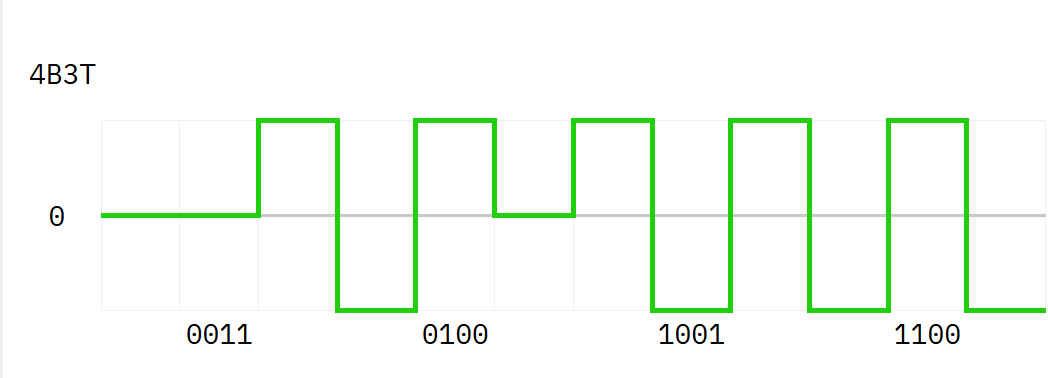
\includegraphics[width=0.9\linewidth,trim={2 0 0 0},clip]{4b3t-example.png}
  \label{fig:4b3t-exemplo}
\end{figure}

O 4B3T opera a uma taxa de símbolo de 120 kbaud para transmitir a taxa total de 160 kbps (dados e controle), considerando que cada símbolo transporta efetivamente $4/3 \approx 1{,}33$ bits de informação. Este valor reduzido de baud rate contribui para minimizar a atenuação de alta frequência e a interferência externa, tornando o esquema particularmente adequado para enlaces de longa distância sem repetidores.

\subsection{Vantagens e limitações}

Entre as principais vantagens do 4B3T destaca-se sua alta eficiência espectral, que permite transmissões robustas sobre par trançado convencional sem necessidade de equalização complexa ou regeneração de sinal. Um sinal codificado utilizando o código de linha 4B3T pode ser transmitido por até 4,2 km em cabos com 0.4 mm de diâmetro, ou até 8,2 km em cabos com 0.6 mm de diâmetro, o que demonstra que não são necessários ajustes avançados para que a transmissão percorra longas distâncias.

Adicionalmente, a estrutura balanceada da codificação reduz o conteúdo de baixa frequência no sinal transmitido, possibilitando o uso de acoplamento por transformadores sem distorções significativas. Isto é fundamental para garantir compatibilidade eletromagnética (EMC) e imunidade a interferências de modo comum.

Contudo, o código 4B3T também apresenta limitações. A principal refere-se à maior sensibilidade a ruído, dado que o sistema depende da correta detecção de três níveis distintos em condições de canal ruidoso. A menor distância entre níveis comparativamente a esquemas binários tradicionais requer uma relação sinal-ruído (SNR) mais elevada para assegurar taxas de erro aceitáveis.

Por fim, embora o mapeamento busque minimizar o DC offset, a variabilidade temporal da componente contínua não é completamente eliminada, podendo exigir técnicas adicionais de correção em cenários mais exigentes.

\section{Código de linha 8B6T}

\subsection{Contextualização e aplicações}

A codificação 8B6T (eight binary, six ternary) surge no contexto da evolução das redes Ethernet em direção a velocidades de 100 Mb/s, especificamente no padrão 100BASE-T4. Essa tecnologia foi concebida com o objetivo de aproveitar a infraestrutura de cabeamento de par trançado de categoria 3, comum em instalações de telefonia e redes locais legadas. A proposta era permitir a migração de redes 10BASE-T para Fast Ethernet sem a necessidade de substituição do cabeamento existente, que não suportaria modulações de maior complexidade espectral exigidas por padrões como o 100BASE-TX, que requerem cabos de categoria 5.

Diferentemente de outras variantes que dependem de codificações intermediárias combinadas com esquemas de modulação subsequentes, como é o caso da codificação 4B5B seguida por MLT-3 no 100BASE-TX, a codificação 8B6T atua diretamente como um esquema de codificação de linha. Isso significa que a transformação de dados binários em sinais transmitidos no meio físico é realizada exclusivamente por essa codificação, sem a necessidade de modulação adicional. O 8B6T é particularmente relevante no contexto do 100BASE-T4 por permitir uma representação eficiente de dados binários utilizando símbolos ternários com três níveis de tensão (positivo, negativo e zero), reduzindo a exigência de largura de banda e permitindo o controle do componente de corrente contínua (DC) da linha, algo crítico em meios balanceados como os utilizados em cabeamento telefônico.

\subsection{Funcionamento}

O funcionamento da codificação 8B6T baseia-se na conversão de blocos de 8 bits binários em sequências de 6 símbolos ternários, cada um assumindo valores entre -1, 0 ou +1, o que caracteriza uma modulação por amplitude de pulso com três níveis (PAM-3). A razão para a escolha dessa codificação está na relação entre o número de combinações possíveis de 6 símbolos ternários, que é de 729 (\(3^6\)), e o número de combinações de 8 bits binários, que é de 256 (\(2^8\)). Isso gera um excesso de 473 combinações possíveis que não são diretamente mapeadas para padrões binários e podem, portanto, ser exploradas para outros propósitos, como a detecção de erros, o controle de sincronismo e, sobretudo, o balanceamento de polaridade da linha de transmissão. A codificação utiliza uma tabela de mapeamento (lookup-table) cuidadosamente construída, na qual cada sequência binária de 8 bits é associada a uma sequência ternária específica com propriedades bem definidas. Uma parte da tabela de mapeamento pode ser observado na Tabela \ref{tab:8b6t}.

\begin{table}[ht]
\centering
\caption{Parte da tabela de codificação 8B6T}
\renewcommand{\arraystretch}{1.2}
\setlength{\tabcolsep}{6pt}
\begin{tabular}{cc|cc|cc}
\toprule
\textbf{Dados} & \textbf{Código} & \textbf{Dados} & \textbf{Código} & \textbf{Dados} & \textbf{Código} \\
\midrule
\texttt{0x00} & \texttt{-+00-+} & \texttt{0x20} & \texttt{-++-00} & \texttt{0x40} & \texttt{-00+0+} \\
\texttt{0x01} & \texttt{0-+-+0} & \texttt{0x21} & \texttt{+00+--} & \texttt{0x41} & \texttt{0-00++} \\
\texttt{0x02} & \texttt{0-+0-+} & \texttt{0x22} & \texttt{-+0-++} & \texttt{0x42} & \texttt{0-0+0+} \\
\texttt{0x03} & \texttt{0-++0-} & \texttt{0x23} & \texttt{+-0-++} & \texttt{0x43} & \texttt{0-0++0} \\
\texttt{0x04} & \texttt{-+0+0-} & \texttt{0x24} & \texttt{+-0+00} & \texttt{0x44} & \texttt{-00++0} \\
\texttt{0x05} & \texttt{+0--+0} & \texttt{0x25} & \texttt{-+0+00} & \texttt{0x45} & \texttt{00-0++} \\
\texttt{0x06} & \texttt{+0-0-+} & \texttt{0x26} & \texttt{+00-00} & \texttt{0x46} & \texttt{00-+0+} \\
\texttt{0x07} & \texttt{+0-+0-} & \texttt{0x27} & \texttt{-+++--} & \texttt{0x47} & \texttt{00-++0} \\
\texttt{0x08} & \texttt{-+00+-} & \texttt{0x28} & \texttt{0++-0-} & \texttt{0x48} & \texttt{00+000} \\
\texttt{0x09} & \texttt{0-++-0} & \texttt{0x29} & \texttt{+0+0--} & \texttt{0x49} & \texttt{++-000} \\
\bottomrule
\end{tabular}
\label{tab:8b6t}
\end{table}

Cada sequência ternária selecionada a partir da tabela possui uma ponderação, que representa a diferença entre o número de níveis positivos e negativos. As ponderações possíveis nas sequências mapeadas diretamente da tabela são 0 ou +1, evitando-se intencionalmente ponderações negativas. Isso é essencial para garantir a previsibilidade e controle do componente DC do sinal transmitido. O processo de transmissão inicia-se com a linha em estado de ponderação neutra (zero). Quando uma sequência com ponderação 0 é transmitida, não há alteração no estado da linha. Ao se transmitir uma sequência com ponderação +1, o estado da linha é atualizado para +1. Se uma nova sequência com ponderação +1 for selecionada enquanto a linha ainda estiver nesse estado, ela é invertida, trocando-se os sinais positivos por negativos e vice-versa, o que gera uma sequência de ponderação -1. Essa inversão reequilibra a linha, retornando o estado de ponderação a zero.

O receptor, ao identificar uma sequência com ponderação -1, reconhece que se trata de uma inversão e aplica o processo inverso, restaurando a sequência original antes de realizar a decodificação binária. Esse mecanismo assegura que, ao longo do tempo, a quantidade de sinais positivos e negativos permaneça aproximadamente equilibrada, o que reduz ou elimina o componente de corrente contínua do sinal (DC offset), contribuindo para a integridade do sinal transmitido. O controle de sincronismo é também favorecido pela escolha cuidadosa das sequências ternárias, que asseguram transições regulares no sinal e permitem a identificação robusta de padrões válidos e de erros simples.

A Figura \ref{fig:8b6t-example} ilustra um exemplo de transmissão da sequência de bytes \texttt{0x00}, \texttt{0x22}, \texttt{0x09} e \texttt{0x42} utilizando o esquema de codificação 8B6T. Inicialmente, o byte \texttt{0x00} é transmitido com o padrão de sinais \texttt{-+00-+}, cuja ponderação é 0, mantendo o estado de equilíbrio da linha em 0. Em seguida, transmite-se o byte \texttt{0x22}, codificado pelo sinal \texttt{-+0-++}, com ponderação +1, alterando o estado da linha de 0 para +1. No terceiro passo, envia-se o byte \texttt{0x09}, codificado no padrão \texttt{0-++-0}, com ponderação 0. Note que, embora o estado da linha esteja em +1, o sinal é transmitido sem inversão, devido a sua ponderação neutra. Por fim, transmite-se o byte \texttt{0x42}, codificado originalmente como \texttt{0-0+0+}, com ponderação +1. No entanto, devido ao estado da linha ser +1, aplica-se a inversão do sinal, resultando no padrão \texttt{0+0-0-}, com ponderação -1. Isso restaura o estado da linha para 0 e mantém o balanço do componente DC.   

\begin{figure}[ht]
  \centering
  \caption{Exemplo de codificação 8B6T}
  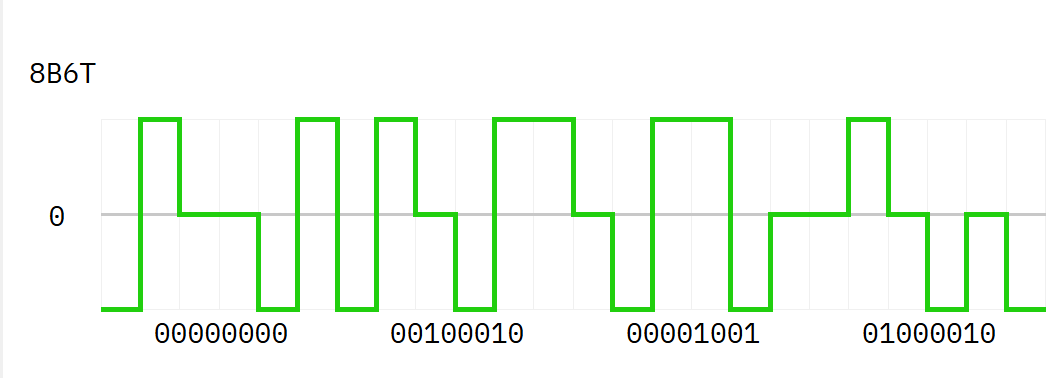
\includegraphics[width=0.9\linewidth,trim={2 0 0 0},clip]{8b6t-example.png}
  \label{fig:8b6t-example}
\end{figure}

\subsection{Vantagens e limitações}

A codificação 8B6T oferece elevada eficiência espectral ao transmitir 8 bits de informação com apenas 6 símbolos ternários, resultando em uma taxa de 1,33 bits por símbolo. Essa eficiência permite operar em cabeamentos de categoria 3, que possuem menor largura de banda disponível e maior suscetibilidade a ruídos, sem comprometer a integridade do sinal (MOLLE; WATSON, 1996). Além disso, o uso de três níveis de sinal favorece o controle do componente DC e o balanceamento da polaridade ao longo do tempo.

Por outro lado, o sistema impõe desafios notáveis. A codificação exige uma tabela extensa para mapear as combinações válidas, aumentando a complexidade de implementação em hardware. Ademais, o 100BASE-T4 opera exclusivamente em half-duplex e requer todos os quatro pares do cabo, em contraste com o 100BASE-TX, que alcança full-duplex utilizando apenas dois pares em cabos de categoria 5. Essas limitações restringiram sua adoção e contribuíram para a rápida obsolescência da tecnologia, à medida que infraestruturas mais modernas tornaram-se economicamente viáveis.

\section{Código de linha 4D-PAM5}

\subsection{Contextualização e aplicações}

O código de linha 4D-PAM5 (Four-Dimensional 5-level Pulse Amplitude Modulation) representa uma evolução na transmissão de dados em alta velocidade, desenvolvido inicialmente para atender às crescentes demandas de largura de banda em redes locais. Este esquema de codificação emergiu no final da década de 1990 como resposta à necessidade de transmitir dados a taxas superiores a 100 Mbps em cabos de cobre convencionais, sem exigir uma completa reestruturação da infraestrutura de cabeamento existente.

A implementação mais notória do 4D-PAM5 encontra-se no padrão 1000BASE-T (Gigabit Ethernet sobre par trançado categoria 5), especificado na norma IEEE 802.3ab. Este padrão revolucionou as redes locais ao permitir transmissões simultâneas bidirecionais (full-duplex) a 1 Gb/s sobre quatro pares de fios de cobre, utilizando cabos Cat5e ou superiores, com alcance de até 100 metros. É adotado em infraestruturas de redes corporativas, acadêmicas e residenciais, constituindo um dos padrões mais implementados na camada física de redes Ethernet contemporâneas.

Além do 1000BASE-T, o esquema 4D-PAM5 ou suas variações encontram aplicabilidade em outros contextos, como em backplanes de alta velocidade, interconexões em data centers e, mais recentemente, como base para desenvolvimentos em padrões como o 2.5GBASE-T e 5GBASE-T, que estendem as capacidades de transmissão em cabeamento estruturado legado.

\subsection{Funcionamento}

O código 4D-PAM5 fundamenta-se na modulação por amplitude de pulso (PAM) utilizando cinco níveis distintos de tensão: -2, -1, 0, +1 e +2, representados frequentemente em volts normalizados. A denominação "4D" refere-se à utilização simultânea de quatro dimensões físicas - neste caso, quatro pares independentes de condutores - para transmissão paralela dos símbolos PAM5.

Diferentemente dos esquemas de codificação binária tradicional, onde cada símbolo transmitido representa um bit (0 ou 1), no PAM5 cada símbolo pode assumir um entre cinco valores possíveis, permitindo a codificação de $\log_2(5) \approx 2{,}32$ bits por símbolo. Contudo, como 2,32 não é um número inteiro, o esquema de codificação utiliza uma abordagem mais sofisticada: em vez de codificar cada símbolo individualmente, o 4D-PAM5 opera sobre grupos de oito bits, mapeando-os para quatro símbolos PAM5 (um para cada par de condutores), resultando em uma eficiência de codificação de $8 \text{ bits} / 4 \text{ símbolos} = 2 \text{ bits por símbolo}$.


No padrão 1000BASE-T, cada par de fios transmite a 125 Mbaud (mega símbolos por segundo). Com quatro pares operando simultaneamente e cada símbolo representando efetivamente 2 bits de informação, atinge-se uma taxa de transferência agregada de 4 × 125 × 2 = 1000 Mb/s, ou 1 Gbps. Este cálculo, entretanto, simplifica o processo real, que inclui bits adicionais para controle de erro, sincronização e outras funções auxiliares.

O processo de codificação envolve inicialmente a conversão dos dados de entrada em blocos de 8 bits. Estes blocos são então codificados em vetores 4D (quádruplas) de símbolos PAM5, seguindo um mapeamento específico que maximiza a distância euclidiana entre pontos adjacentes no espaço 4D, otimizando assim a imunidade a ruído (AZADET et al., 2001). 

O sistema emprega um scrambler pseudoaleatório baseado em um registrador de deslocamento (LFSR) de 33 bits, utilizando o polinômio gerador padrão \( G(x) = x^{33} + x^{13} + 1 \). A sequência gerada (\( 2^{33} - 1 \) períodos) é aplicada via operação XOR aos bits de dados, distribuindo a energia espectral de forma uniforme e reduzindo componentes de corrente contínua (DC). A natureza determinística do scrambler permite ao receptor reconstruir a sequência original mediante a sincronização do estado inicial, sem comprometer a integridade dos dados.


Adicionalmente, incorpora-se um esquema de modulação denominado TCM (Trellis Coded Modulation). Usualmente a implementação do TCM no 4D-PAM5 utiliza um codificador convolucional que adiciona um bit redundante aos 8 bits de dados, totalizando 9 bits por símbolo. Esse bit adicional particiona a constelação 4D em duas famílias (par/ímpar), restringindo os símbolos válidos a subconjuntos específicos. Como resultado, a distância mínima entre símbolos válidos aumenta (\(d_2 = 4\)), proporcionando um ganho de aproximadamente +5,2 dB na margem de erro através da decodificação de Viterbi. Essa redundância é viável graças à elevada cardinalidade da constelação 4D-PAM5: das 625 combinações possíveis (\(5^4\)), apenas 256 são utilizadas para dados, permitindo ter 100\% de redundância alêm de sobrar 113 símbolos para controle. Na nossa implementação, utilizamos uma versão simplificada do bit de redundância, onde adicionamos a paridade do dado original com base na operação XOR. A Figura \ref{fig:4D-PAM5-full-duplex} ilustra um exemplo de codificação 4D-PAM5.

Um dos principais aspectos do 4D-PAM5 no contexto do 1000BASE-T é sua capacidade de suportar operação full-duplex em cada par de fios. Isto é possível através da implementação de circuitos de cancelamento de eco, que permitem a cada extremidade filtrar sua própria transmissão do sinal recebido, isolando assim o sinal proveniente do dispositivo remoto.

\begin{figure}[ht]
  \centering
  \caption{Exemplo de codificação 4D‑PAM5}
  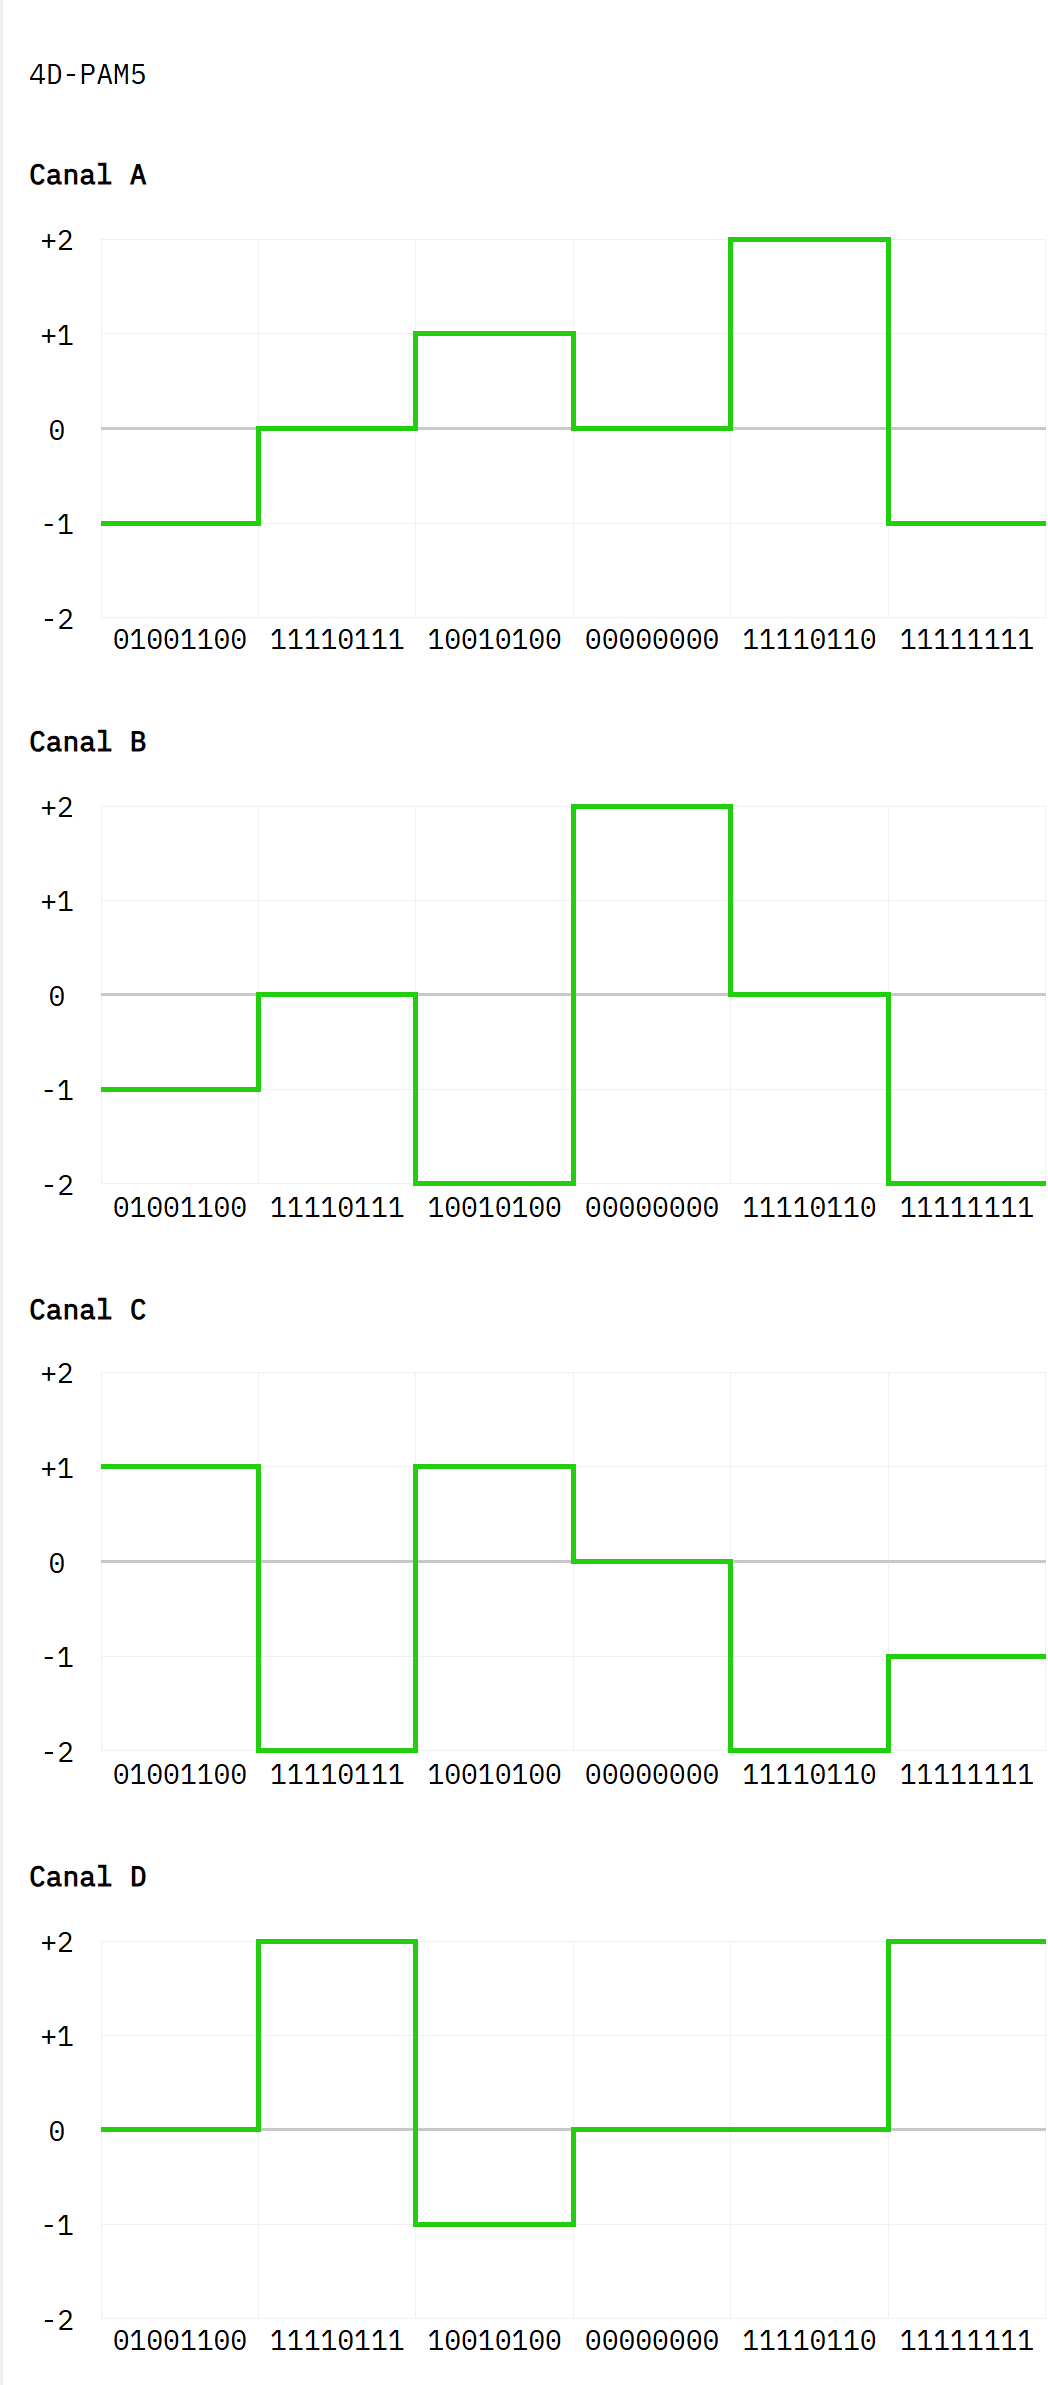
\includegraphics[width=0.9\linewidth,trim={3 0 0 0},clip]{4dpam5-example.png}
  \label{fig:4D-PAM5-full-duplex}
\end{figure}

\subsection{Vantagens e limitações}

O esquema 4D-PAM5 apresenta vantagens que justificam sua adoção em comunicações de alta velocidade. Primeiramente, sua eficiência espectral superior, como supracitado, permite transmissões a 1 Gbps em cabos de cobre convencionais, sem necessidade de expansão da largura de banda ocupada comparativamente aos padrões anteriores como o 100BASE-TX. Esta característica viabilizou a migração para Gigabit Ethernet sem substituição massiva da infraestrutura de cabeamento instalada.

Em segundo lugar, a codificação 4D-PAM5 implementada no padrão 1000BASE-T apresenta robustez contra interferências eletromagnéticas, graças à incorporação de técnicas de processamento de sinais como o TCM e a equalização adaptativa. Estas técnicas, aliadas ao cancelamento de eco, permitem operação confiável mesmo em ambientes com elevado ruído elétrico.

Adicionalmente, o código apresenta distribuição espectral favorável, com componente DC reduzida, facilitando o acoplamento através de transformadores e minimizando problemas relacionados à interferência intersimbólica (ISI). A utilização de cinco níveis de amplitude, em vez de apenas dois como em códigos binários convencionais, permite reduzir a frequência fundamental do sinal transmitido, relaxando os requisitos de largura de banda do meio físico (GRIFFITHS, 2017).

Apesar de suas vantagens, o 4D-PAM5 também apresenta limitações. A principal refere-se à maior suscetibilidade a ruídos em comparação com esquemas binários. Como os cinco níveis de amplitude estão mais próximos entre si, a margem de erro é menor, exigindo uma relação sinal-ruído (SNR) mais elevada para manter a taxa de erro dentro de limites aceitáveis. Ou seja, a maior eficiência espectral é obtida às custas de uma menor robustez intrínseca ao ruído.

Além disso, a implementação do 4D-PAM5 é mais complexa. Requer circuitos de codificação e decodificação sofisticados, bem como subsistemas para cancelamento de eco, equalização e recuperação de temporização. Isso implica maior demanda de processamento digital de sinais, consumo energético mais elevado e custos aumentados, além de possíveis impactos na latência.

Por fim, o 4D-PAM5 também apresenta maior sensibilidade a imperfeições do canal, como descontinuidades de impedância e diafonia (crosstalk) entre pares adjacentes. Estas características impõem requisitos quanto à qualidade dos componentes utilizados na infraestrutura de cabeamento, incluindo conectores, cabos e interfaces de rede.

\section{Conclusão}

Os códigos de linha 4B3T, 8B6T e 4D-PAM5 evidenciam diferentes estratégias para otimizar a transmissão de dados em meios físicos limitados, abordando aspectos como eficiência espectral, controle de componente DC e robustez frente a ruídos. Enquanto o 4B3T e o 8B6T destacam-se pela adaptação a infraestruturas legadas com soluções de codificação ternária, o 4D-PAM5 representa um avanço significativo ao permitir transmissões gigabit em cabeamentos de categoria 5, ainda que à custa de maior complexidade de implementação. Cada técnica analisada demonstra como os requisitos de aplicação influenciam diretamente o projeto dos esquemas de codificação de linha.


\begin{thebibliography}{00}


\bibitem{ProakisSalehi2008}
PROAKIS, J. G.; SALEHI, M. Digital Communications. 5ª ed. Nova York: McGraw-Hill, 2008.

\bibitem{Sklar2001}
SKLAR, B. Digital Communications: Fundamentals and Applications. 2ª ed. Upper Saddle River: Prentice Hall, 2001.


\bibitem{}
AZADET, K. et al. Equalization and FEC techniques for optical transceivers. IEEE Journal of Solid-State Circuits, v. 37, n. 3, p. 317-327, 2001.

\bibitem{}
GRIFFITHS, D. J. Introduction to Electrodynamics. 4ª ed. Cambridge: Cambridge University Press, 2017.

\bibitem{}
HATAMIAN, M. et al. Design considerations for gigabit ethernet 1000BASE-T twisted pair transceivers. Proceedings of the IEEE Custom Integrated Circuits Conference, p. 335-342, 1998.

\bibitem{}
IEEE. IEEE 802.3ab: 1000BASE-T Specification. IEEE Standards Association, 1999.

\bibitem{}
SEIFERT, R.; EDWARDS, J. The All-New Switch Book: The Complete Guide to LAN Switching Technology. 2ª ed. Indianapolis: Wiley Publishing, 2008.

\bibitem{}
STALLINGS, W. Data and Computer Communications. 10ª ed. Upper Saddle River: Pearson, 2013.

\bibitem{}
TANENBAUM, A. S.; WETHERALL, D. Redes de Computadores. 5ª ed. São Paulo: Pearson, 2011.

\bibitem{}
INTERNATIONAL TELECOMMUNICATION UNION. Recommendation I.430: Basic user-network interface - Layer 1 specification. Genebra: ITU-T, 1995.

\bibitem{}
EUROPEAN TELECOMMUNICATIONS STANDARDS INSTITUTE. ETR 080: Transmission and Multiplexing (TM); Integrated Services Digital Network (ISDN) basic rate access; Digital transmission system on metallic local lines. Sophia Antipolis: ETSI, 1991.

\bibitem{}
STARR, T.; CIOFFI, J. M.; SILVERMAN, P. J. Understanding Digital Subscriber Line Technology. 1ª ed. Upper Saddle River: Prentice Hall, 1999.

\bibitem{}
SPURGEON, C. E.; ZIMMERMAN, J. Ethernet: The Definitive Guide. Sebastopol, Ca: O’reilly, 2014. 

\bibitem{}
SEIFERT, R. Gigabit Ethernet. [s.l.] Addison-Wesley Professional, 1998. 

\bibitem{}
FOROUZAN, B. A.; FEGAN, S. C.. Data communications and networking. ª. ed. New York: McGraw-Hill, 2006.


\bibitem{}
MOLLE, M.; WATSON, G. 100Base-T/IEEE 802.12/packet switching. IEEE Communications Magazine, v. 34, n. 8, p. 64–73, 1 jan. 1996.

\end{thebibliography}

\end{document}
